\subsection{Rancangan Detail Komponen}
\label{subsection:detail-komponen}

Berdasarkan rancangan struktural yang sudah dijelaskan pada bagian \ref{subsection:rancangan-struktural}, sistem akan diimplementasikan sebagai kumpulan komponen. Masing-masing komponen tersebut memiliki peran dan tanggung jawab yang berbeda dalam sistem eksperimen. Pada bagian ini, akan dijelaskan lebih lanjut mengenai rancangan detail dari masing-masing komponen tersebut.

\subsubsection{Rancangan Detail Node}
\label{subsubsection:detail-node}

Seperti yang sudah dijelaskan pada Bagian \ref{subsubsection:node}, \textit{Node} merupakan satuan fungsional utama yang berperan sebagai entitas dalam sistem \textit{database} terdistribusi yang dikembangkan. Selain komponen yang telah disebutkan pada bagian tersebut, \textit{Node} juga memiliki komponen internal yang berfungsi untuk menghasilkan data \textit{trace} yang dapat digunakan untuk keperluan \textit{debugging} dan analisis kinerja sistem serta konfigurasi yang mengatur perilaku \textit{Node}. Ilustrasi struktur \textit{Node} yang lebih detail dapat dilihat pada Gambar \ref{fig:node-structure}.

Komponen internal lain dalam \textit{Node} adalah jalur komunikasi \textit{message passing} antara antarmuka \textit{client}, antarmuka antar-\textit{Node}, dan komponen konsensus. Hal ini disebabkan karena modularitas implementasi OmniPaxos yang tidak mengintegrasikan komponen konsensus dengan antarmuka jaringan.

Implementasi \textit{erasure coding} bukan terdapat pada \textit{Node} melainkan pada komponen OmniPaxos. Alasan untuk hal ini adalah kompleksitas perubahan dari konsensus yang perlu dilakukan ketika operasi diubah menjadi menggunakan \textit{erasure coding}. Dengan demikian, komponen OmniPaxos akan menangani operasi \textit{erasure coding} dan replikasi data, sementara \textit{Node} akan menerima hasil dari OmniPaxos untuk melanjutkan operasi ke penyimpanan data dan komunikasi antar-\textit{Node}. Detail implementasi \textit{erasure coding} akan dibahas pada Bagian \ref{subsubsection:detail-komponen-konsensus}.

\begin{figure}[ht]
    \centering
    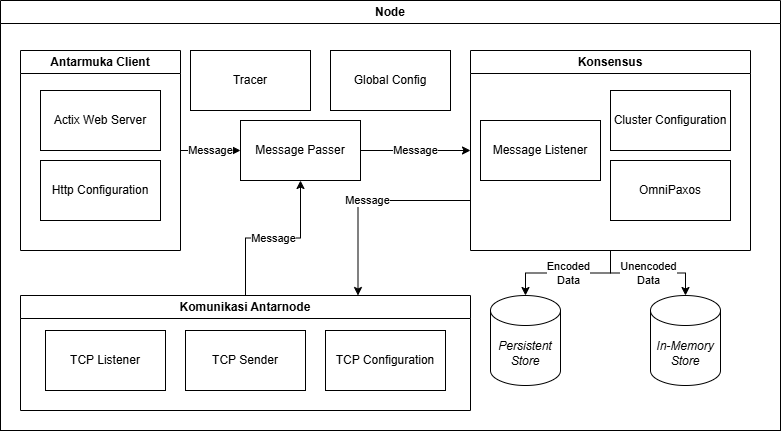
\includegraphics[width=0.95\textwidth]{resources/chapter-3/node-architecture.png}
    \caption{Struktur Node}
    \label{fig:node-structure}
\end{figure}

\subsubsection{Rancangan Detail Subsistem Penyimpanan}
\label{subsubsection:detail-subsistem-penyimpanan}

Subsistem penyimpanan adalah subsistem yang bertanggung jawab untuk fungsionalitas \textit{key-value store} dalam sebuah \textit{Node}. Subsistem ini akan terdiri atas komponen \textit{in-memory store}, \textit{persistent store}, \textit{transaction log}. Subsistem ini juga mengkonfigurasi \textit{Node} untuk menggunakan replikasi atau \textit{erasure coding}.

Mengikuti solusi yang sudah dipilih pada bagian \ref{subsection:alternatif-solusi}, subsistem penyimpanan bersifat modular dengan Moka sebagai \textit{in-memory key-value store} dan RocksDB sebagai \textit{persistent storage}. Pada rancangannya, dalam satu perangkat akan memiliki implementasi \textit{in-memory key-value store} dengan Moka untuk tiap \textit{Node} yang ada. Sementara itu, RocksDB dapat dijalankan pada tiap node tanpa memerlukan \textit{server}.

Ilustrasi struktur subsistem penyimpanan dapat dilihat pada gambar \ref{fig:storage-subsystem-structure}.

% _TODO: Change image
\begin{figure}[ht]
    \centering
    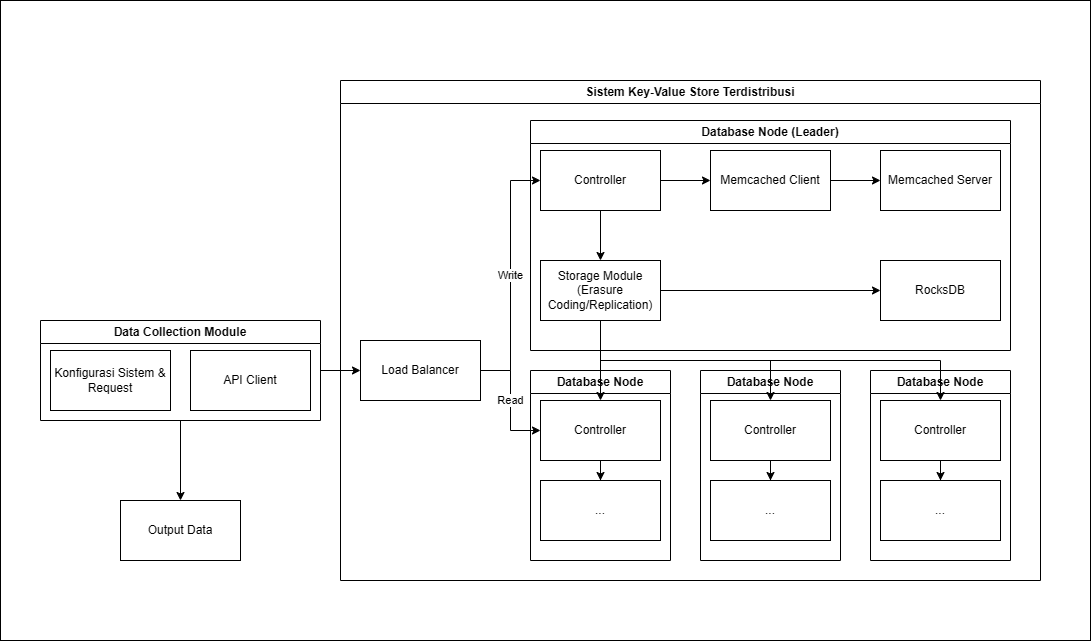
\includegraphics[width=0.95\textwidth]{resources/chapter-3/general-architecture.png}
    \caption{Struktur Subsistem Penyimpanan}
    \label{fig:storage-subsystem-structure}
\end{figure}

\subsubsection{Rancangan Detail Subsistem Kontrol}
\label{subsubsection:detail-subsistem-kontrol}
  
Subsistem Kontrol bertanggung jawab mengelola transaksi dan konsistensi antar-\textit{Node}. Pengelolaan tersebut dilakukan dengan mengaplikasikan algoritma konsensus untuk menjaga konsistensi data antar-\textit{Node}. Subsistem ini juga bertanggung jawab untuk melakukan \textit{recovery} data dari \textit{transaction log} jika terjadi kegagalan pada \textit{Node}.

% TODO: Implementasi paxos better masuk bab 2?
Untuk menjaga konsistensi dari data, subsistem kontrol mengimplementasikan algoritma konsensus untuk tiap transaksinya. Algoritma yang dipakai adalah algoritma \textit{Paxos} karena algoritma ini bersifat transaksional dan \textit{message passing} dan bukan \textit{log replication} sehingga lebih ideal untuk sistem yang menggunakan \textit{erasure coding}.

Pada algoritma \textit{Paxos} yang diimplementasikan, dibuat sebuah mekanisme \textit{leader election}. Modifikasi penambahan \textit{leader election} mempercepat transaksi dengan melewati tahap \textit{propose} pada \textit{Paxos} dengan mengasumsikan bahwa \textit{leader} selalu memiliki nilai yang lebih tinggi dibanding \textit{node} lainnya. Keberadaan \textit{leader} juga mempermudah pembagian \textit{value} hasil operasi \textit{erasure coding}. Nilai ini disebar pada tahap \textit{accept} pada algoritma \textit{Paxos} dan mengembalikan operasi sukses pada \textit{client}.

% TODO: Review, agak aneh ini karena kalo kayak gini konsistensinya agak rendah?
% Tahap \textit{learn} dilakukan dengan penambahan \textit{broadcast} satu kali dari \textit{leader} untuk mengaktifkan nilai yang sudah diterima.


Ilustrasi struktur subsistem kontrol dapat dilihat pada gambar \ref{fig:control-subsystem-structure}.

% _TODO: Change image
\begin{figure}[ht]
    \centering
    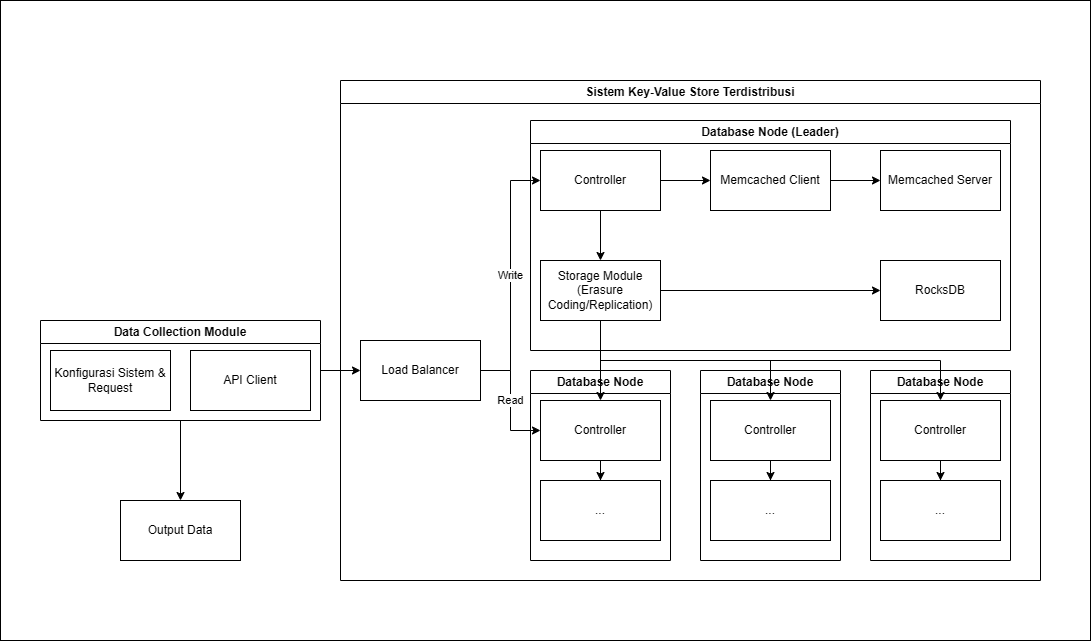
\includegraphics[width=0.95\textwidth]{resources/chapter-3/general-architecture.png}
    \caption{Struktur Subsistem Kontrol}
    \label{fig:control-subsystem-structure}
\end{figure}
\subsubsection{Rancangan Detail Komponen HTTP Server}
\label{subsubsection:detail-komponen-HTTP-server}

Komponen HTTP \textit{server} berfungsi sebagai antarmuka komunikasi antara \textit{client} dan \textit{Node}. Komponen ini bertanggung jawab untuk menerima dan memproses permintaan dari \textit{client}, serta mengirimkan respons yang sesuai.

Ilustrasi struktur komponen HTTP \textit{server} dapat dilihat pada gambar \ref{fig:http-server-structure}.

% _TODO: Change image
\begin{figure}[ht]
    \centering
    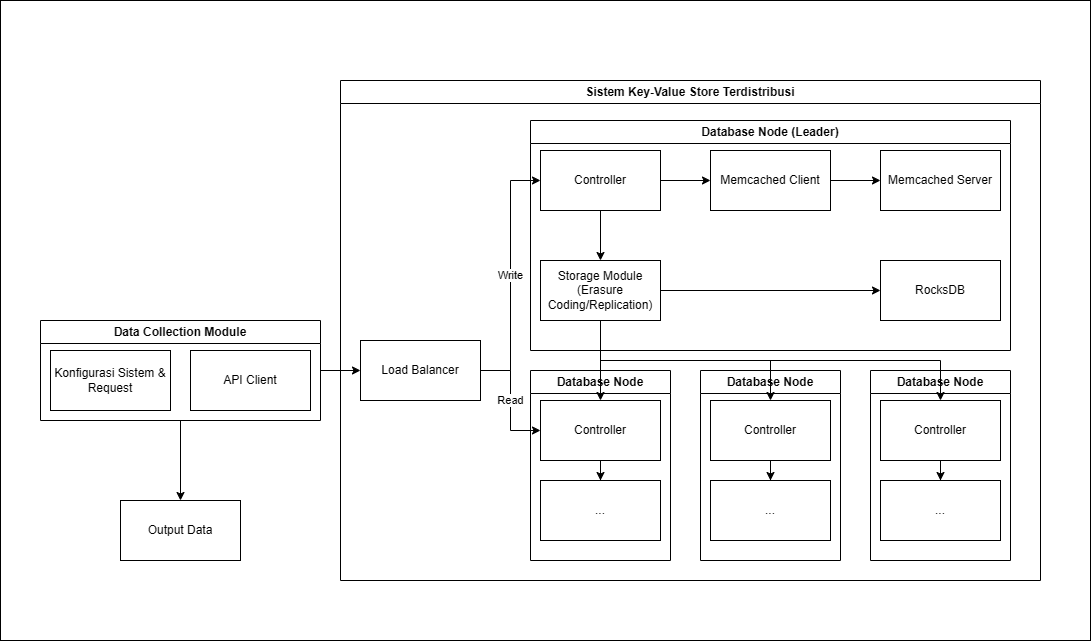
\includegraphics[width=0.95\textwidth]{resources/chapter-3/general-architecture.png}
    \caption{Struktur Komponen HTTP Server}
    \label{fig:http-server-structure}
\end{figure}

\subsection{Rancangan Detail Komponen Komunikasi Antar-Node}
\label{subsection:detail-subsistem-komunikasi-antar-node}

Komponen komunikasi antar-\textit{Node} bertanggung jawab untuk mengelola komunikasi antar-\textit{Node} dalam sistem terdistribusi. Komponen ini akan menggunakan protokol komunikasi yang sesuai untuk memastikan bahwa data dapat dikirim dan diterima.

Ilustrasi struktur komponen komunikasi antar-\textit{Node} dapat dilihat pada gambar \ref{fig:node-communication-structure}.

% _TODO: Change image
\begin{figure}[ht]
    \centering
    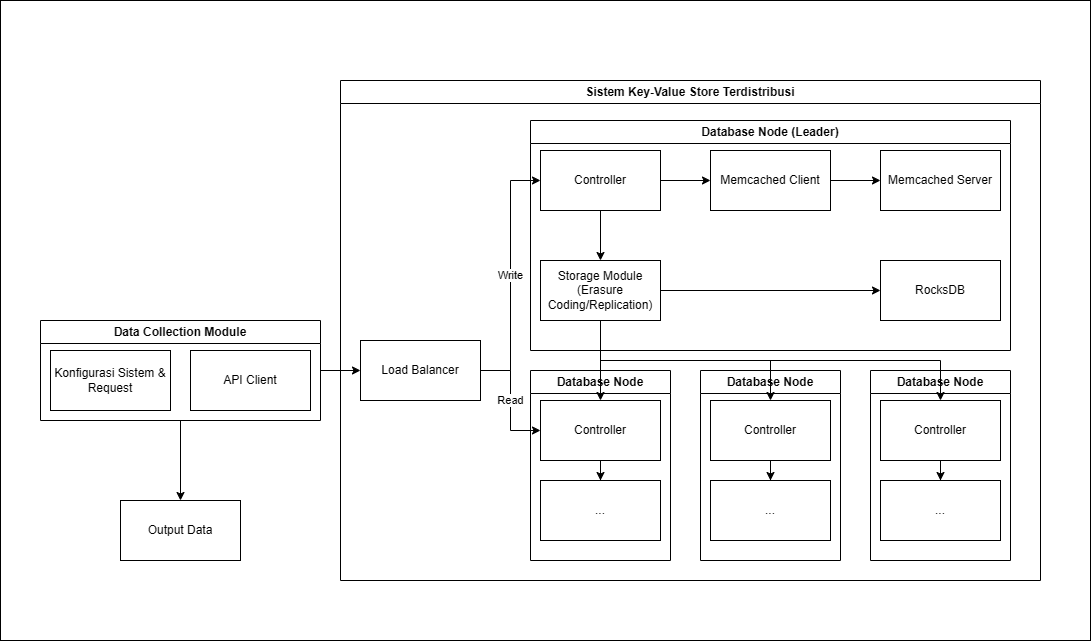
\includegraphics[width=0.95\textwidth]{resources/chapter-3/general-architecture.png}
    \caption{Struktur Komponen Komunikasi Antar-Node}
    \label{fig:node-communication-structure}
\end{figure}
\subsubsection{Rancangan Detail Data Collector}
\label{subsubsection:detail-data-collector}

Data Collector adalah komponen yang bertanggung jawab untuk mengumpulkan data dari sistem dan menyimpannya dalam format yang sesuai untuk analisis lebih lanjut. Komponen ini akan mengumpulkan data dari berbagai sumber, termasuk log sistem, metrik kinerja, dan informasi lainnya yang relevan.
Data Collector juga akan menyediakan antarmuka untuk mengakses data yang telah dikumpulkan, sehingga memudahkan pengguna untuk melakukan analisis dan visualisasi data.

Struktur \textit{Data Collector} terdiri dari:

\begin{enumerate}
    \item Komponen testing: Komponen ini bertanggung jawab untuk melakukan \textit{request} dan transaksi pada sistem.
    \item Komponen \textit{logging} dan \textit{tracing}: Komponen ini mengelola pencatatan dan pelacakan operasi yang dilakukan oleh sistem secara keseluruhan.
    \item Komponen \textit{reporting}: Komponen ini bertanggung jawab untuk mengumpulkan dan menyajikan hasil eksperimen dalam bentuk laporan.
\end{enumerate}

Ilustrasi struktur Data Collector dapat dilihat pada gambar \ref{fig:data-collector-structure}.

% _TODO: Change image
\begin{figure}[ht]
    \centering
    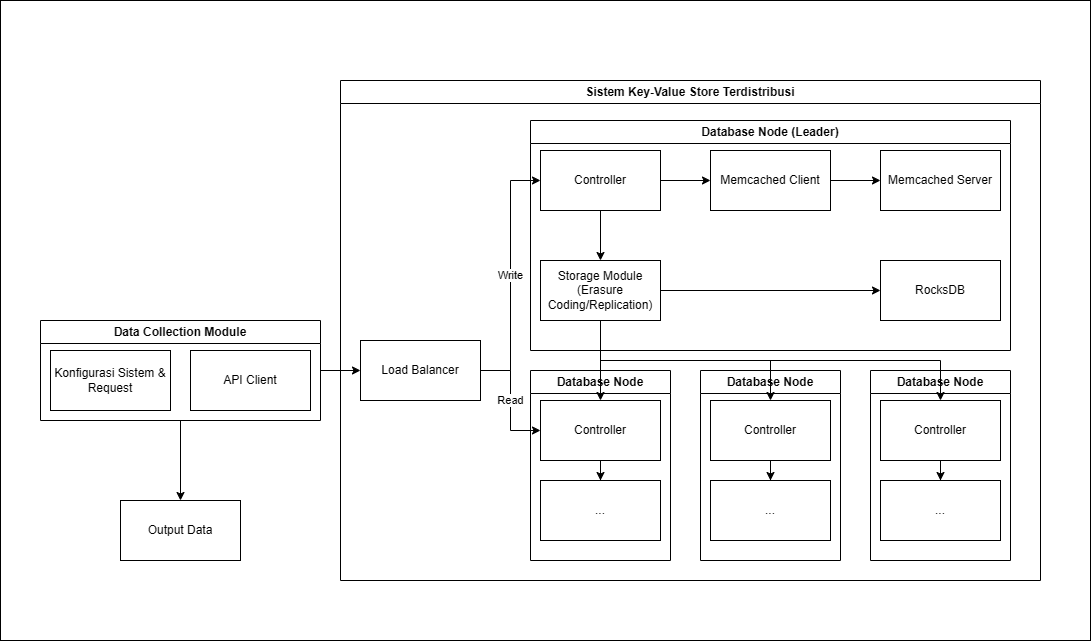
\includegraphics[width=0.95\textwidth]{resources/chapter-3/general-architecture.png}
    \caption{Struktur Data Collector}
    \label{fig:data-collector-structure}
\end{figure}
\subsubsection{Rancangan Detail Komponen Testing}
\label{subsubsection:detail-data-testing}

Komponen \textit{testing} bertanggung jawab untuk melakukan pengujian terhadap sistem yang telah dibangun. Pengujian ini dilakukan untuk memastikan bahwa sistem berfungsi sesuai dengan spesifikasi yang telah ditentukan. Komponen ini juga bertanggung jawab untuk menghasilkan data yang kemudian dimasukkan ke komponen \textit{reporting} untuk visualisasi dan analisis.

Ilustrasi struktur komponen \textit{testing} dapat dilihat pada gambar \ref{fig:testing-structure}.

% _TODO: Change image
\begin{figure}[ht]
    \centering
    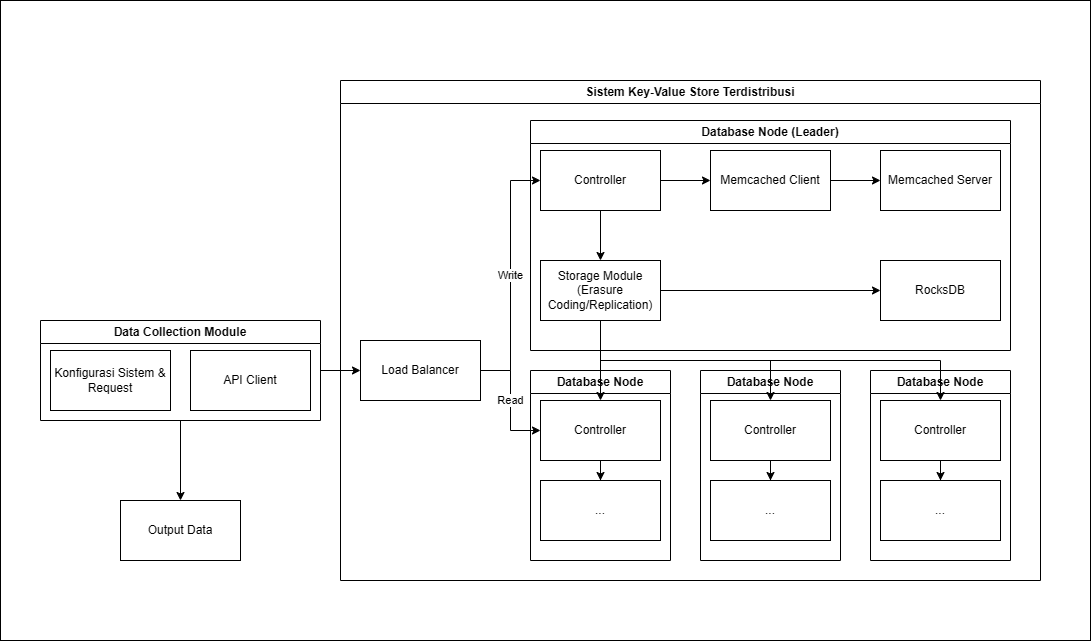
\includegraphics[width=0.95\textwidth]{resources/chapter-3/general-architecture.png}
    \caption{Struktur Komponen Testing}
    \label{fig:testing-structure}
\end{figure}
\subsubsection{Rancangan Detail Komponen Logging}
\label{subsubsection:detail-data-logging}

Komponen \textit{logging} dan \textit{tracing} bertanggung jawab untuk mencatat dan melacak aktivitas sistem. Komponen ini akan mengumpulkan data dari berbagai komponen lain dalam sistem, termasuk informasi tentang permintaan yang diterima, respons yang dikirim, dan status sistem secara keseluruhan. Data ini akan digunakan untuk analisis lebih lanjut dan pemecahan masalah.

Ilustrasi struktur komponen \textit{logging} dan \textit{tracing} dapat dilihat pada gambar \ref{fig:logging-tracing-structure}.

% _TODO: Change image
\begin{figure}[ht]
    \centering
    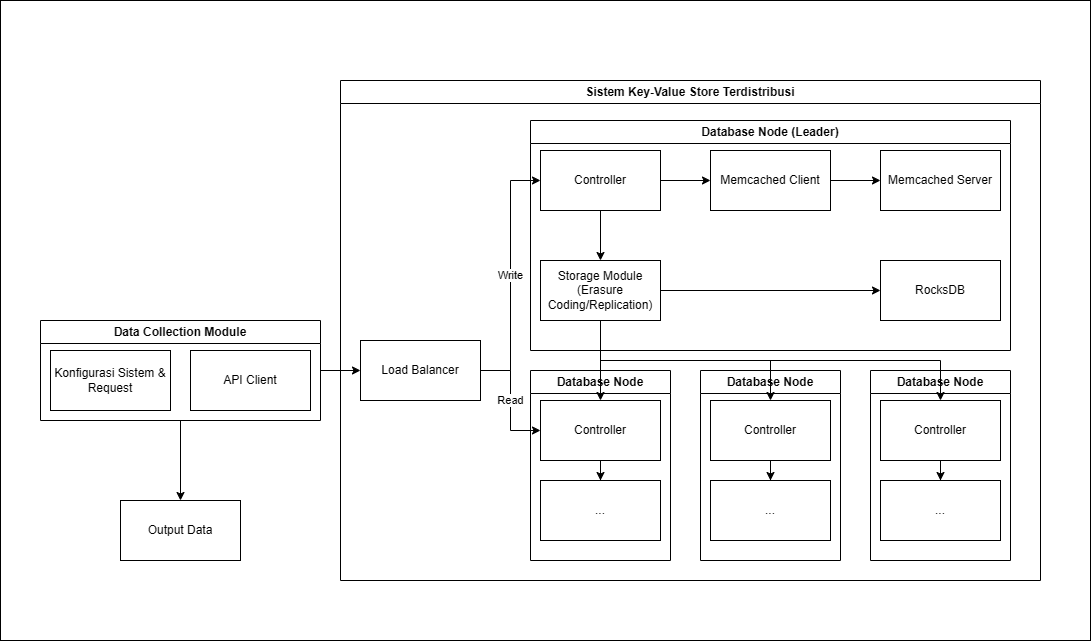
\includegraphics[width=0.95\textwidth]{resources/chapter-3/general-architecture.png}
    \caption{Struktur Komponen Logging dan Tracing}
    \label{fig:logging-tracing-structure}
\end{figure}
